%% Supplementary material for the Briefings in Bioinformatics submission.
%%
%% TWO FACTS FROM J8 SHAPE THIS FILE, and both are recorded in
%% briefings_in_bioinformatics_lock.json -> j8_completion_20260817.supplementary:
%%
%%   1. It IS peer reviewed -- "All material to be considered as supplementary data must be
%%      submitted at the same time as the main manuscript for peer review." So this is not an
%%      appendix nobody reads. It is part of what the referees judge.
%%
%%   2. It is NOT copyedited or typeset -- "Supplementary material will not be copyedited or
%%      typeset, and it will be available online upon publication." So what we hand over is exactly
%%      what a reader sees, forever. It is compiled as a standalone document for that reason, and
%%      it is held to the same standard as the main text rather than used as a dumping ground.
%%
%% Supplementary figures and tables are normal here, not a concession: of the three BiB papers
%% sampled, all three carry supplementary material and one (SurvBoard, bbaf521) carries
%% supplementary methods, Figs S1-S5 and Tables S1-S3.
%%
%% Figures are NOT copied into this directory. \graphicspath points at where they are built.

\documentclass[11pt]{article}
\usepackage[utf8]{inputenc}
\usepackage[T1]{fontenc}
\usepackage{geometry}
\geometry{a4paper, margin=2.5cm}
\usepackage{graphicx}
\graphicspath{{../figures/}}
\usepackage{afterpage}
\usepackage{booktabs}
\usepackage{longtable}
\usepackage{amsmath}
\usepackage[numbers,sort&compress]{natbib}
\usepackage[hidelinks]{hyperref}
\usepackage{xcolor}

\newcommand{\TODOport}[1]{\textcolor{red}{\textbf{[TODO: }#1\textbf{]}}}

%% S-numbering, which is what the journal's own papers use ("Supplementary Fig. 5A",
%% "Supplementary Table S1").
\renewcommand{\thefigure}{S\arabic{figure}}
\renewcommand{\thetable}{S\arabic{table}}
\renewcommand{\theequation}{S\arabic{equation}}
\renewcommand{\thesection}{S\arabic{section}}

\title{Supplementary material\\[0.3em]
\large ModRank: parameter-free fusion of histology, transcriptome and pathologic stage
for bladder cancer survival}
\date{}

%% article.cls sets the TOC section-number box to 1.5em, which two-digit
%% section numbers overrun. Same definition, one dimension widened.
\makeatletter
\renewcommand*\l@section[2]{%
  \ifnum \c@tocdepth >\z@
    \addpenalty\@secpenalty
    \addvspace{1.0em \@plus\p@}%
    \setlength\@tempdima{2.2em}%
    \begingroup
      \parindent \z@ \rightskip \@pnumwidth
      \parfillskip -\@pnumwidth
      \leavevmode \bfseries
      \advance\leftskip\@tempdima
      \hskip -\leftskip
      #1\nobreak\hfil
      \nobreak\hb@xt@\@pnumwidth{\hss #2\kern-\p@\kern\p@}\par
    \endgroup
  \fi}
\makeatother

%% FLOAT PLACEMENT, chosen by measuring body ink per page across four configurations rather
%% than by looking. The defaults reserve 20%% of every page for text, which in a supplement whose
%% floats are full-width figures pushed the last reference onto a page of its own at 8.6%% fill.
%% Measured 2026-08-20: defaults 11 pages with an 8.6%% page, a \clearpage before the bibliography
%% 11 pages with a 15.4%% page, both together 11 pages with two thin pages, and these four
%% parameters 10 pages whose only page under 0.79 is the last one, where the document ends.
\renewcommand{\topfraction}{0.95}
\renewcommand{\bottomfraction}{0.7}
\renewcommand{\textfraction}{0.07}
\renewcommand{\floatpagefraction}{0.75}

\begin{document}
\maketitle
\tableofcontents
\newpage

\section{The clinical-baseline census, one paper at a time}

The manuscript's central claim is a claim about other people's papers, so it has to be checkable one
row at a time. This is that extraction (Table~\ref{tab:sup-census}). \textbf{A row says ``verified'' only where
the covariate sentence was read in the paper itself}. Where it was not, the row says so and why, rather than
being filled in from what the other rows suggest.

\begin{table}[h]
\centering
{\small
\begin{tabular}{llll}
\toprule
paper & venue & clinical baseline & stage? \\
\midrule
PORPOISE / MMF~\cite{chen2022porpoise} & Cancer Cell 2022 & age, gender, tumour grade & \textbf{no stage} \\
SurvPath~\cite{jaume2024survpath} & CVPR 2024 & age, sex, grade & \textbf{no stage} \\
PIBD~\cite{zhang2024pibd} & ICLR 2024 & \emph{reports no clinical baseline} & n/a \\
MOTCat~\cite{xu2023motcat} & ICCV 2023 & \emph{reports no clinical baseline} & n/a \\
MMP~\cite{song2024mmp} & ICML 2024 & age, sex, cancer grade & \textbf{no stage} \\
DIMAF~\cite{eijpe2025dimaf} & MICCAI 2025 & grade, age, sex & \textbf{no stage} \\
OTSurv~\cite{ren2025otsurv} & MICCAI 2025 & \emph{reports no clinical baseline} & n/a \\
DSCASurv~\cite{song2025dscasurv} & Briefings in Bioinformatics 26 & \emph{reports no clinical baseline} & n/a \\
MCAT~\cite{chen2021mcat} & ICCV 2021 & \emph{not verified} & n/a \\
MOAD-FNet~\cite{moadfnet2024} & arXiv 2024 & \emph{not verified} & n/a \\
APL~\cite{apl2025} & arXiv 2025 & \emph{not verified} & n/a \\
\bottomrule
\end{tabular}}
\caption{Every method paper associated with this benchmark, and what it compares against. Of the
8 we read, \textbf{4 report a clinical-variable baseline and every one of them builds it from
grade}. \textbf{Not one uses pathologic stage}, and \textbf{4 report no clinical baseline at all}.
3 could not be verified and are marked as such.}
\label{tab:sup-census}
\end{table}

\noindent The verbatim covariate statements behind the four ``verified'' rows of
Table~\ref{tab:sup-census}:
\begin{itemize}
  \item \textbf{PORPOISE / MMF}: ``we also assessed Cox proportional hazard models using age, gender, and tumor grade covariates as baselines, which were still outperformed by MMF (Table S4)'' (main text, referring to Table S4, 'Cox Baselines on Survival Prediction across 14 Cancer Types')
  \item \textbf{SurvPath}: ``Age, Sex, Grade'' (Supplementary Table 3)
  \item \textbf{MMP}: ``The clinical baseline includes age, sex, and cancer grade as reported in the TCGA cohort.'' (Table 1 caption)
  \item \textbf{DIMAF}: ``multivariate linear Cox regression as a clinical baseline using grade, age, and sex'' (Table 1, 'Clinical' row)
\end{itemize}

\noindent \textbf{The half that reports nothing is the sharper half.} Four of the eight papers we
read compare against no clinical variable at all. Their baselines are other deep-learning models
only. On this benchmark the comparison against the clinic is therefore either made against a
covariate that cannot work in this disease, or never made.

\section{Why grade cannot separate patients in this disease}
\begin{table}[h]
\centering
{\small
\setlength{\tabcolsep}{4pt}
\begin{tabular}{lcccccccc}
\toprule
 & & \multicolumn{3}{c}{grade} & \multicolumn{3}{c}{stage} & \\
\cmidrule(lr){3-5}\cmidrule(lr){6-8}
study & $n$ & levels & modal & entropy & levels & modal & entropy & stage $-$ grade \\
\midrule
BLCA (bladder) & 359 & 2 & 94.4\% & 0.311 & 5 & 50.6\% & 0.665 & $+0.0560$ \\
BRCA & 871 & \multicolumn{3}{c}{no usable grade in the shipped file} & 5 & 60.3\% & 0.631 & $+0.0858$ \\
COADREAD & 298 & \multicolumn{3}{c}{no usable grade in the shipped file} & 5 & 68.7\% & 0.572 & $+0.2208$ \\
HNSC & 394 & 5 & 59.7\% & 0.643 & 5 & 37.5\% & 0.884 & $+0.0423$ \\
STAD & 319 & 4 & 58.9\% & 0.623 & 4 & 47.3\% & 0.835 & $+0.0461$ \\
\bottomrule
\end{tabular}}
\caption{Level composition and normalised Shannon entropy of the two covariates, in each of the five
studies the benchmark covers, and the gain from swapping one for the other. \textbf{Source: every
row here uses SurvPath's own released clinical files}, which is the only clinical source
that exists for all five studies. The bladder headline in the main text ($0.6638$ against $0.5666$,
$+0.0972$) is a \emph{different} construction (it takes every column from DIMAF's own released split files, which is what makes it a statement about the incumbent's own baseline) and on
bladder this table's source gives $+0.0560$ instead. Neither is derived from the other and both are
internal to one pipeline on one set of cases. \textbf{Two studies ship no usable grade}: for BRCA
and COADREAD the ``grade'' arm is age and sex alone, so there the comparison shows stage improving
that baseline rather than stage beating grade. They are marked rather than dropped, because
dropping them would make a five-study claim rest on three.}
\label{tab:sup-entropy}
\end{table}

\noindent Table~\ref{tab:sup-entropy} sets the two covariates side by side in every study.
Bladder is the extreme case and the reason the defect matters most here: two
grade levels with 94.4\% of cases in one of them. A covariate that does not distinguish the
patients cannot separate them, whatever model is fitted on top of it.

\section{The frozen protocol, and its one amendment}
The frozen protocol fixes the arm, the estimator, the alpha
grid, the combination rule, the comparator set, the seeds and the decision rule, and it was written
after the falsifiers ran and before the confirmatory run. The rule as written was: primary
$> 0.679 + 0.0239$ \emph{and} standard deviation across seeds $\leq 0.0145$, where 0.0239 is
$\sigma\sqrt{2\ln N}$ evaluated at the 211 candidates the ledger held at the moment of writing.
Both conditions are met and the first of them is mis-specified, which the main paper reports and
Section~\ref{sec:campaign} below returns to.

\paragraph{Amendment A1 had two effects, and they pull in opposite directions.} Fixing the defect (a cached clinical query had taken the \emph{first} of several diagnosis records per case, and 61 of 359 changed once the correct record was chosen) is worth $+0.0050$ on ModRank. Rebuilding
the block from the incumbent's own four columns also \emph{drops} the T, N and M our cached query
had supplied, which is worth $-0.0110$. Net, the reported primary fell from 0.7260 to
\textbf{0.7212}, a move of $-0.0048$ and the same size as the seed-to-seed SD. We report the lower,
more conservative arm. It clears the bar the pre-registered rule set, 0.7029, and does not clear
the bar that rule would have set had its selection term been specified correctly.

The tell was present and unread before the check: Stage IIA, IIB and IIC appear in that cached
record and are not AJCC bladder stages at all.

\section{The falsifier that was built wrong the first time}
All five leakage falsifiers, their thresholds and their outcomes are in the Methods, where two of
the five rejected. One of them needed rebuilding and that is what this section records, because a
falsifier that fires is worth nothing if the reason it fired was the falsifier. The planted-label
construction was wrong on the first attempt: a single column built for the whole cohort encoded the outcome on every training row as
well as every validation row, because each case sits in exactly one validation fold, and it
reported a 0.8715 ``leak'' that did not exist. Rebuilt per fold it moves the score by $-0.0006$.

\section{The development campaign, and what its size does and does not license}
\label{sec:campaign}
The development campaign scored $N=269$ candidate arms, in a ledger generated from the runs' own
output rather than kept by hand.

\paragraph{The frozen rule was written against a smaller campaign than the one that ran.} The
protocol records its selection term at $N=211$, giving 0.0239 and the pre-registered target of
0.7029, and 211 is what the ledger held at the moment the protocol was written. Two further
sub-experiments, 58 rows between them, were scored afterwards and still before the confirmatory
run, taking the campaign to 269. The same term over 269 gives 0.0244 for a bar of 0.7034, which the
reported 0.7212 also clears. The undercount is recorded here rather than left for a reader to find
by opening the protocol, and it runs in the direction that makes the frozen bar the more permissive
of the two.

The main paper reports why the term is wrong for a reason that has nothing to do with $N$: the
$\sigma$ substituted into it is the spread of a paired between-arm difference, and the expression
needs the spread of a candidate's own absolute score. This section records what the ledger does
support.

\paragraph{Not all 269 are candidates the frozen arm competed against.} A rank is only meaningful
among values comparable to it, and four kinds of row are not. The error atlas contributes 26
subgroup slices, each scored on part of the cohort. A further 18 are in-sample oracles, fitted and
scored on the same rows on purpose, to measure what a given capacity can memorise. Another 14 are
permuted or null controls, built to lose and reported as the thing their partner had to beat, and 5
are cross-cohort transfer probes scored on a different disease. That leaves \textbf{206}
full-cohort out-of-fold values, and the five parts sum to 269 by construction rather than by
assertion.

\paragraph{The maximum was not taken, which is what the correction assumes.} Among those 206 the
frozen configuration is rank \textbf{11}, counting every tied row against it. Eight distinct
configurations score strictly above: two are a different TCGA study, three are components this
paper rejects on their own pre-registered controls, and the rest are the declared transcriptomic
sensitivity. The two remaining places are the frozen construction's own duplicates, which the
ledger records three times because three sub-experiments arrived at it independently and each
logged it under its own name. Reporting the optimistic rank of 9 would have been defensible and we
report the pessimistic one.

This narrows what a maximum-of-$N$ correction means here. It does not rescue the rule, and the
main paper does not use it to.

\section{Seven falsified components, each with the control read before its result}
\begin{table}[h]
\centering
{\small
\begin{tabular}{cllccl}
\toprule
 & component & predicted & observed & control & status \\
\midrule
C1 & pan-cancer survival subspace prior & $+0.0300$ & $-0.0042$ & $-0.0141$ & void \\
C1$'$ & the same direction, zero-shot & $+0.0250$ & $+0.0033$ & $-0.0311$ & void \\
C2 & bagged ridge & $+0.0400$ & $-0.0561$ & n/a & graded \\
C4 & dense regularisation path & $+0.0200$ & $-0.0042$ & n/a & void \\
C5 & gated fusion on clinical risk & $+0.0200$ & $+0.0046$ & $+0.0055$ & void \\
C6 & inner-CV skill weighting & $+0.0200$ & $+0.0105$ & n/a & void \\
C7 & stratified partial likelihood & $+0.0300$ & $-0.0199$ & $-0.0095$ & graded \\
\bottomrule
\end{tabular}}
\caption{The seven components. Every \emph{predicted} value in Table~\ref{tab:sup-components} was fixed before the run. The bar is
0.0145, twice the measured split-reseed SD. None cleared it.}
\label{tab:sup-components}
\end{table}

\noindent Figure~\ref{fig:sup-campaign} draws the same campaign three ways. Panels a and b are this
table, the predicted against the observed and then the four components that carry a matched
control. Panels c and d are the five-study generalisation both halves at once. Panels e and f are
the seven-encoder sweep, which is what settles whether the lead belongs to the method or to its
slide encoder.

\begin{figure}[h]
\centering
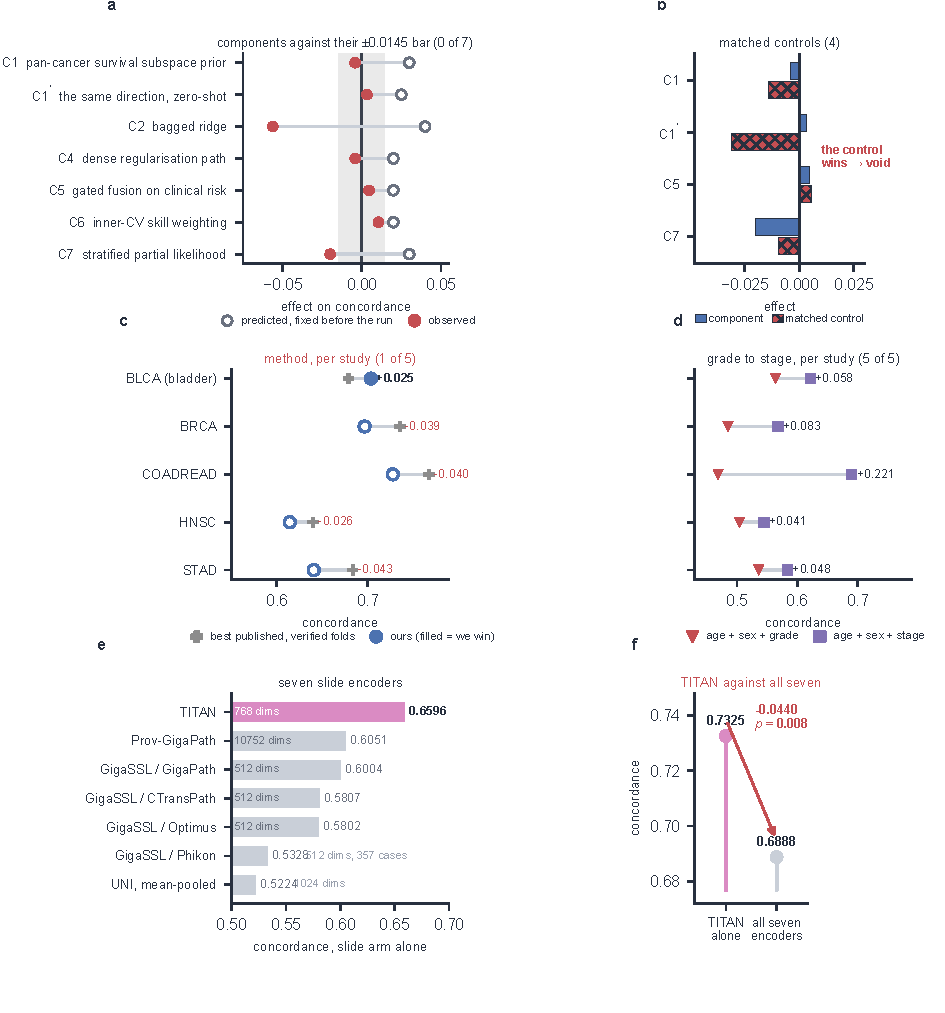
\includegraphics[width=\textwidth]{figS1_campaign.pdf}
\caption{\textbf{The development campaign, its generalisation and its representations.}
\textbf{(a)} What each of the seven components was predicted to be worth, fixed before the run,
against what it was worth. The shaded band is the $\pm0.0145$ bar and none cleared it.
\textbf{(b)} The four that carry a matched control. C5's control beats it, which is what a void
looks like. \textbf{(c)} ModRank against the best published entry with verified folds, per study:
bladder wins, four of five lose. \textbf{(d)} The one-column swap in the same five studies, five of
five. Both halves of the generalisation are here because reporting only the second would make a
claim the paper declines to make. \textbf{(e)} Seven slide encoders scored as single arms on
identical cases and folds. \textbf{(f)} The seven-encoder pool against TITAN alone, paired on
cases, significantly worse ($-0.0440$, $p=0.008$).}
\label{fig:sup-campaign}
\end{figure}

\section{Per-seed and per-fold numbers}
The primary is a mean over five seeds and the seeds move it, so the individual values are given
rather than summarised. Table~\ref{tab:sup-perseed} is every arm at every seed, and it is what the
three concordances the main text distinguishes are reconstructed from.

\begin{table}[h]
\centering
{\small
\begin{tabular}{ccccc}
\toprule
seed & ours & slide & omics & clinical \\
\midrule
0 & 0.7225 & 0.6596 & 0.6510 & 0.6638 \\
1 & 0.7248 & 0.6515 & 0.6733 & 0.6657 \\
2 & 0.7129 & 0.6550 & 0.6470 & 0.6638 \\
3 & 0.7243 & 0.6553 & 0.6664 & 0.6644 \\
4 & 0.7216 & 0.6472 & 0.6681 & 0.6666 \\
\midrule
mean & \textbf{0.7212} & & & \\
SD & 0.0048 & & & \\
\bottomrule
\end{tabular}}
\caption{Every arm at every seed, so that three quantities the main text keeps distinct (the
primary 0.7212, the seed-0 value 0.7225, and the concordance of the seed-averaged score vector,
0.7237) can each be reconstructed rather than believed.}
\label{tab:sup-perseed}
\end{table}


\section{The two case-selection rules}

Two case series were specified in the analysis files before either was run, and \textbf{neither
replaced the other}. Both draw from the same band (the middle tertile of the clinical arm's out-of-fold risk, 119 patients) because that is where a model is being asked to add something to
the stage.

\begin{itemize}
  \item \textbf{Series A, ten cases.} The five highest and five lowest full-method scores in the
    band. Reported in the Results.
  \item \textbf{Series B, twelve cases.} The four highest and four lowest full-method scores, plus
    the two largest slide-over-omics and two largest omics-over-slide disagreements. Drawn in
    Figure~7e of the main paper, because a score ranking alone hides the cases where the two
    molecular-facing arms contradict each other.
\end{itemize}

Every case either rule admits is reported, including the ones that embarrass the model, such as the up-revised
patient censored at 2.2 months in Series B, and the single down-revised event in
Series A. An earlier draft of this supplement described Series A as a superseded version of
Series B. That was wrong, and it is corrected here rather than silently: they are concurrent series
answering different questions, and describing one as an earlier version of the other would have
implied a rule change that never happened.


\section{Three corrections made during the study}
\paragraph{The oracle control answered the wrong question.} An in-sample oracle was compared against
a control that fitted permuted outcomes and scored the \emph{real} ones. That measures whether two
different targets are related, not how much a fit is inflated by being scored on the outcomes it was
fitted to, so it answers about 0.5 at any capacity. The corrected null (fit the permuted outcome, score \emph{that same} permutation) reaches \textbf{0.7474} at sixteen parameters. Two numbers
read off the first control, an ``estimation loss'' of 0.1170 and a ``recoverable'' 0.2686, are
withdrawn. What triggered the recheck was not suspicion: component C2 had pre-registered that
variance reduction would help each arm in proportion to its dimension, and it failed in the opposite
direction.

\paragraph{The planted-label falsifier was wrong on its first construction.} One column built for
the whole cohort put the outcome ordering on every row, training rows included, because each case
sits in exactly one validation fold. It reported a 0.8715 ``leak'' that did not exist. Rebuilt per
fold it moves the score by $-0.0006$.

\paragraph{Our own clinical block was defective.} Described above as amendment A1.

\paragraph{Two of the three moved the reported number down, and all three are in the paper.} A
correction that only ever improves the result is a correction worth being suspicious of.

\section{The full pathway landscape, and what each molecular arm tracks}

The main text reports the fifteen strongest of 275 pathways, which is the favourable tail of
the distribution. Figure~\ref{fig:sup-landscape} is all of them. The headline is negative and it belongs in
the record: \emph{no} pathway clears Benjamini--Hochberg $q<0.10$ as a univariate predictor of
disease-specific survival in this cohort, so whatever the transcriptomic arm contributes it does
not contribute through any single programme. Panel b carries the less expected result. The slide arm
and the transcriptomic arm agree only moderately about \emph{patients}, sharing Spearman 0.48
between their out-of-fold scores, yet their pathway-association profiles correlate at $r=0.82$.
They disagree about which patient is at risk far more than they disagree about which biology is
associated with risk, which is a different statement from either arm being a subtype reader.

\begin{figure}[t]
\centering
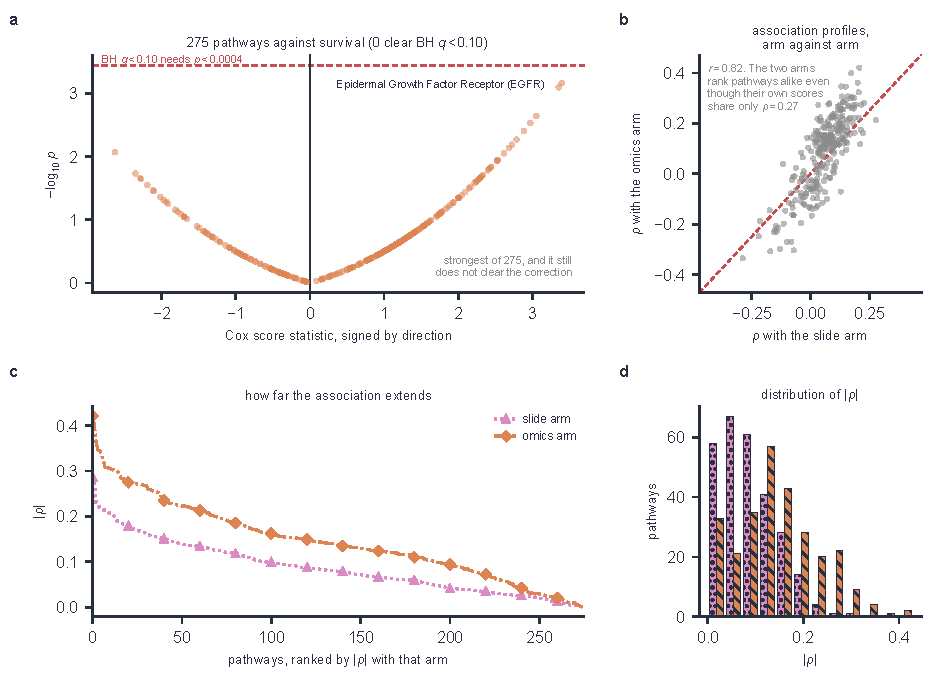
\includegraphics[width=\textwidth]{figS4_pathway_landscape.pdf}
\caption{\textbf{All 275 pathways.} \textbf{(a)} Univariate Cox score statistic against $-\log_{10}
p$, signed by whether the pathway scores above or below chance as a raw risk score, which is the
direction convention used in the main text. The dashed rule is the smallest $p$ that would clear
Benjamini--Hochberg at $q<0.10$, and nothing reaches it. \textbf{(b)} Each pathway's Spearman
correlation with the slide arm against its correlation with the transcriptomic arm.
\textbf{(c, d)} How far the association extends, ranked and binned.}
\label{fig:sup-landscape}
\end{figure}

\section{Per-fold behaviour and calibration}

Five folds is a small number and the released partition is not balanced in events: fold~5 carries
16 of the 113 against 23 to 25 elsewhere. Figure~\ref{fig:sup-perfold} reports what the pooled
number hides. ModRank's concordance spans \textbf{0.678 to 0.782} across the five folds, a range of
\textbf{0.103}, against a standard deviation of 0.0048 across seeds. Fold-to-fold variation is an
order of magnitude larger than seed variation, and it is larger than every margin reported on this
benchmark including our own. This is the same conclusion the power analysis reaches in the main
text, arrived at from a different direction, and it is the reason we decline to treat the ordering
of the published table as resolved.

The score is nonetheless calibrated in the ordinary sense: binning cases by ModRank percentile and
reading observed Kaplan--Meier survival at 22 months gives a monotone decreasing curve across all
five bins, from 0.89 in the lowest to 0.42 in the highest. Tertile separation holds within every
fold separately, not only after pooling.

\begin{figure}[t]
\centering
\includegraphics[width=\textwidth]{figS5_perfold_calibration.pdf}
\caption{\textbf{Per fold, and calibrated.} \textbf{(a)} Concordance within each fold, per arm.
\textbf{(b)} Kaplan--Meier by ModRank tertile with the cuts taken within each fold, so no fold
borrows another's thresholds. \textbf{(c)} Observed survival at 22 months against ModRank
percentile bin. \textbf{(d)} Out-of-fold score distributions pooled across folds. \textbf{(e)} Cases
and events per fold.}
\label{fig:sup-perfold}
\end{figure}

\bibliographystyle{plain}
\bibliography{../references}

\end{document}
